\documentclass[conference]{IEEEtran}
\IEEEoverridecommandlockouts
\usepackage{cite}
\usepackage{amsmath,amssymb,amsfonts}
\usepackage{algorithm}
\usepackage{algpseudocode}
\usepackage{graphicx}
\usepackage{booktabs}
\usepackage{multirow}
\usepackage{textcomp}
\usepackage{xcolor}
\usepackage{tikz}
\usetikzlibrary{arrows.meta,positioning,fit,calc}
\usepackage{fancyhdr}

% ---- course header on every page ----
\newcommand{\groupno}{2}
\fancypagestyle{uct}{%
  \fancyhf{}%
  \fancyhead[L]{\scriptsize Group No.: \groupno \quad Project Name: INN-RC (Lossless Image Steganography)}%
  \fancyhead[R]{\scriptsize Reetam Dutta (102318024), Priyadarshi Vivekanand (102318048)}%
  \fancyfoot[C]{\scriptsize\thepage}%
  \renewcommand{\headrulewidth}{0.3pt}}
\setlength{\headheight}{12pt}

\newcommand{\R}{\mathbb{R}}
\newcommand{\Z}{\mathbb{Z}}
\newcommand{\ablA}{2747}
\newcommand{\ablB}{1869}
\newcommand{\ablC}{1589}
\newcommand{\ablD}{497}
\newcommand{\ablDicomC}{15325}
\newcommand{\ablDicomD}{2150}
\newcommand{\ablRatio}{5.5}
\newcommand{\ablRatioNb}{3.2}
\newcommand{\auxBASE}{111.7k}
\newcommand{\auxQeight}{365}
\newcommand{\auxQfour}{561}
\newcommand{\auxQtwo}{1659}
\newcommand{\auxRatio}{199}
\newcommand{\auxReight}{429}
\newcommand{\auxRfour}{610}
\newcommand{\auxRtwo}{928}
\newcommand{\berinnQeight}{0.44}
\newcommand{\berinnQfour}{3.04}
\newcommand{\berinnQtwo}{7.34}
\newcommand{\berinnReight}{0.23}
\newcommand{\berinnRfour}{2.05}
\newcommand{\berinnRtwo}{4.19}
\newcommand{\capPEE}{9.6k}
\newcommand{\exactBASE}{0}
\newcommand{\exactPEE}{393}
\newcommand{\exactQ}{385}
\newcommand{\exactR}{371}
\newcommand{\failBASE}{132}
\newcommand{\failPEE}{3}
\newcommand{\failQ}{11}
\newcommand{\failR}{25}
\newcommand{\nImgs}{132}
\newcommand{\okBASE}{0}
\newcommand{\okPEE}{393}
\newcommand{\okQ}{385}
\newcommand{\okR}{371}
\newcommand{\pinnBASE}{46.07}
\newcommand{\pinnQeight}{50.16}
\newcommand{\pinnQfour}{49.40}
\newcommand{\pinnQtwo}{46.64}
\newcommand{\pinnReight}{49.26}
\newcommand{\pinnRfour}{47.92}
\newcommand{\pinnRtwo}{43.49}
\newcommand{\psnrPEEeight}{71.64}
\newcommand{\psnrPEEfour}{65.32}
\newcommand{\psnrPEEtwo}{57.84}
\newcommand{\psnrQeight}{49.92}
\newcommand{\psnrQfour}{49.05}
\newcommand{\psnrQtwo}{45.73}
\newcommand{\psnrReight}{49.03}
\newcommand{\psnrRfour}{47.57}
\newcommand{\psnrRtwo}{42.94}
\newcommand{\resBASE}{36}
\newcommand{\robgaussonePEE}{50.17}
\newcommand{\robgaussoneQ}{2.07}
\newcommand{\robgaussoneR}{1.26}
\newcommand{\robgaussthreePEE}{50.05}
\newcommand{\robgaussthreeQ}{6.30}
\newcommand{\robgaussthreeR}{3.62}
\newcommand{\robgausstwoPEE}{49.87}
\newcommand{\robgausstwoQ}{3.22}
\newcommand{\robgausstwoR}{1.76}
\newcommand{\robjpegeightyPEE}{50.04}
\newcommand{\robjpegeightyQ}{47.02}
\newcommand{\robjpegeightyR}{46.10}
\newcommand{\robjpegnfPEE}{50.15}
\newcommand{\robjpegnfQ}{12.14}
\newcommand{\robjpegnfR}{5.07}
\newcommand{\robjpegninetyPEE}{50.47}
\newcommand{\robjpegninetyQ}{38.74}
\newcommand{\robjpegninetyR}{36.07}
\newcommand{\robnonezeroPEE}{0.00}
\newcommand{\robnonezeroQ}{1.78}
\newcommand{\robnonezeroR}{1.16}
\newcommand{\robspsphalfPEE}{48.29}
\newcommand{\robspsphalfQ}{3.35}
\newcommand{\robspsphalfR}{2.17}
\newcommand{\robspsponePEE}{48.99}
\newcommand{\robspsponeQ}{6.10}
\newcommand{\robspsponeR}{4.03}
\newcommand{\runsBASE}{132}
\newcommand{\runsPEE}{396}
\newcommand{\runsQ}{396}
\newcommand{\runsR}{396}
\newcommand{\ssimPEEeight}{0.9999}
\newcommand{\ssimPEEfour}{0.9998}
\newcommand{\ssimPEEtwo}{0.9991}
\newcommand{\ssimQeight}{0.9960}
\newcommand{\ssimQfour}{0.9949}
\newcommand{\ssimQtwo}{0.9896}
\newcommand{\ssimReight}{0.9955}
\newcommand{\ssimRfour}{0.9940}
\newcommand{\ssimRtwo}{0.9821}
\newcommand{\tembPEEeight}{0.02}
\newcommand{\tembPEEfour}{0.02}
\newcommand{\tembPEEtwo}{0.02}
\newcommand{\tembQeight}{0.49}
\newcommand{\tembQfour}{0.51}
\newcommand{\tembQtwo}{0.59}
\newcommand{\tembReight}{0.49}
\newcommand{\tembRfour}{0.51}
\newcommand{\tembRtwo}{0.56}
\newcommand{\textPEEeight}{0.02}
\newcommand{\textPEEfour}{0.02}
\newcommand{\textPEEtwo}{0.02}
\newcommand{\textQeight}{0.48}
\newcommand{\textQfour}{0.51}
\newcommand{\textQtwo}{0.59}
\newcommand{\textReight}{0.49}
\newcommand{\textRfour}{0.51}
\newcommand{\textRtwo}{0.56}


\begin{document}

\title{Lossless Image Steganography with a Message-Conditioned Integer Coupling Network and Context-Coded Residual Compensation}

\author{\IEEEauthorblockN{Reetam Dutta}
\IEEEauthorblockA{\textit{Dept. of Computer Science and Engineering}\\
\textit{Thapar Institute of Engineering and Technology}\\
Patiala, India}
\and
\IEEEauthorblockN{Priyadarshi Vivekanand}
\IEEEauthorblockA{\textit{Dept. of Computer Science and Engineering}\\
\textit{Thapar Institute of Engineering and Technology}\\
Patiala, India}}

\maketitle
\thispagestyle{uct}
\pagestyle{uct}

\begin{abstract}
Reversible data hiding returns the cover exactly, but its hidden bits are lost when the stego image is changed; deep
steganography networks are robust, but floating-point rounding stops them from returning the cover. We
propose INN-RC, a lossless steganography scheme built on a message-conditioned integer coupling network (IC-INN). The
cover is split into two pixel halves that are updated in turn by rounded offsets predicted from the other half and the
message, so the receiver can undo the network exactly once it knows the message and no latent variable has to be
stored. A small decoder reads the message back. The bits it gets wrong and the pixels clipped at 0 or 255 are coded with
a context-adaptive arithmetic coder, whose contexts are the decoder confidence and the coupling offset re-estimated by the
receiver, and are hidden with multi-layer rhombus prediction-error expansion. The 62.9k-parameter model trains on a CPU and the
pipeline runs in MATLAB. On \nImgs{} test images from BSD100, Kodak and real DICOM CT/MR/CR scans,
every successfully embedded image was recovered bit for bit with zero bit error rate. At 0.0156 bpp (1024 bits) the
stego PSNR is \psnrQfour{} dB (SSIM \ssimQfour{}) and the side information averages \auxQfour{} bits, about half the
message length, while a float invertible network with the same compensation would need \auxBASE{} bits. Unlike classical
prediction-error expansion, whose bits are lost under any distortion, the message survives Gaussian noise ($\sigma=2$)
and 1\% salt-and-pepper noise with a BER of \robgausstwoR\% and \robspsponeR\%.
\end{abstract}


\begin{IEEEkeywords}
reversible data hiding, steganography, invertible neural network, integer coupling, arithmetic coding, prediction-error expansion
\end{IEEEkeywords}

\section{Introduction}
Steganography hides a message inside an innocent-looking cover so that only the intended receiver knows it is there.
In most deep steganography systems the cover is treated as disposable: the network adds a small perturbation, the
receiver reads the message, and the original image is gone for good. For medical scans, legal evidence, satellite and
military imagery this is not acceptable, because the exact original pixels may be needed later. Reversible data hiding
(RDH) solves the reversibility part. Classical RDH schemes based on difference expansion~\cite{tian2003de}, histogram
shifting~\cite{ni2006hs} and prediction-error expansion (PEE)~\cite{thodi2007pee,sachnev2009,ou2013ppee} return the cover
bit for bit, but the hidden bits are destroyed by the smallest change to the marked image, such as a single JPEG save.

Deep, and in particular invertible, networks have the opposite profile. Invertible steganography networks such as
HiNet~\cite{jing2021hinet} and ISN~\cite{lu2021isn} hide and reveal with the same weights, and noise-layer training as in
HiDDeN~\cite{zhu2018hidden} or RIIS~\cite{xu2022riis} makes the message survive distortion. However, these networks work in
floating point. When the stego image is rounded to 8 bits and the part of the output that is not transmitted (the
latent) is replaced by zeros, the inverse pass no longer gives back the cover. Recent robust-reversible work, DRRW and
CRMark~\cite{chen2025drrw,chen2025crmark}, closes this gap with an \emph{integer} invertible network: overflowed pixels and
the dropped latent are compressed into an auxiliary bitstream and hidden again with classical RDH.

We follow the same two-stage idea but change what has to be stored. Our observation is simple: if the coupling layers
are integer additions that are \emph{conditioned on the message}, then the receiver can undo them exactly as soon as it
knows the message, and there is no latent at all. The message itself is read back by a separate small decoder, and the
only things the receiver can get wrong are (i) a few message bits and (ii) pixels that were clipped at 0 or 255. These
two kinds of residual are what we compensate. Since the decoder outputs a confidence for every bit, the wrong bits are
concentrated where the confidence is low, and an arithmetic coder that uses this confidence as context codes them very
cheaply.

\textbf{Contributions.} The main contributions of this work are:
\begin{itemize}
\item a message-conditioned integer coupling network (IC-INN) whose inverse is exact by construction, so that
exact recovery needs no latent variable, only decoder-error flags and overflow corrections;
\item a residual compensation stage that codes these corrections with a context-adaptive binary arithmetic coder whose
contexts come from the decoder confidence and the local stego values, followed by a multi-layer rhombus PEE embedding
with an overflow-safe predictor range;
\item a lightweight design (62.9k parameters) that trains on a CPU, with a full MATLAB implementation of inference,
coding, embedding, extraction and an App Designer GUI;
\item an evaluation on 132 test images (BSD100, Kodak and real DICOM CT/MR/CR scans) against classical rhombus PEE and a
float-INN baseline with residual compensation, covering exact recovery, image quality, side-information size and
robustness to noise and JPEG.
\end{itemize}

\section{Related Work}
\subsection{Reversible data hiding}
Tian's difference expansion~\cite{tian2003de} and Ni \emph{et al.}'s histogram shifting~\cite{ni2006hs} started spatial
RDH. Thodi and Rodr\'iguez~\cite{thodi2007pee} moved the expansion to prediction errors, and Sachnev
\emph{et al.}~\cite{sachnev2009} improved it with a rhombus predictor, two-pass checkerboard embedding and sorting by local
variance; this is the PEE variant we use in our second stage and as the classical reference. Pairwise PEE~\cite{ou2013ppee}
reduces distortion further by expanding error pairs. Hu and Xiang replaced the hand-made predictor with a CNN
\cite{hu2021cnnp} and added prediction-error-ordering based adaptive embedding \cite{hu2022cnnpami}; Qiu
\emph{et al.}~\cite{qiu2025icnnp} also predict pixel complexity with the network. In all of these, learning only sharpens the
prediction; the hidden bits are not robust.

\subsection{Deep and invertible steganography}
Baluja~\cite{baluja2017} hid a full image inside another with an encoder--decoder CNN, and HiDDeN~\cite{zhu2018hidden}
introduced a noise layer for robust bit hiding. Invertible networks built from affine coupling layers~\cite{dinh2017realnvp}
were then used by HiNet~\cite{jing2021hinet} (in the wavelet domain) and ISN~\cite{lu2021isn} so that hiding and revealing
share all parameters. RIIS~\cite{xu2022riis}, PRIS~\cite{yang2023pris} and Lan \emph{et al.}~\cite{lan2023robust} make the
invertible pipeline robust to distortions and rounding; PRIS in particular points out that rounding errors are usually
ignored in INN steganography. None of these methods returns the cover image.

\subsection{Deep robust reversible watermarking}
DRRW~\cite{chen2025drrw} and CRMark~\cite{chen2025crmark} are the closest to our work. They use an integer invertible
watermark network, in the spirit of integer discrete flows~\cite{hoogeboom2019idf}, map the cover and watermark to an
overflowed stego and a latent, compress both with arithmetic coding and embed the result by RDH. Our scheme differs in
where the message enters: it conditions the integer couplings instead of being one of the network inputs, which removes
the latent from the auxiliary data and lets us use the decoder confidence as coding context.

\section{Proposed Method}
\subsection{Overview}
Fig.~\ref{fig:arch} shows the system. The sender scrambles the message, embeds it with the integer coupling network,
clips the result to 8 bits, measures what the receiver will get wrong, codes these corrections and hides them with PEE.
The receiver runs the same steps backwards. Throughout, $X\in\{0,\dots,255\}^{H\times W}$ is the grayscale cover and
$\mathbf{m}\in\{0,1\}^N$ the message.

\begin{figure*}[t]
\centering
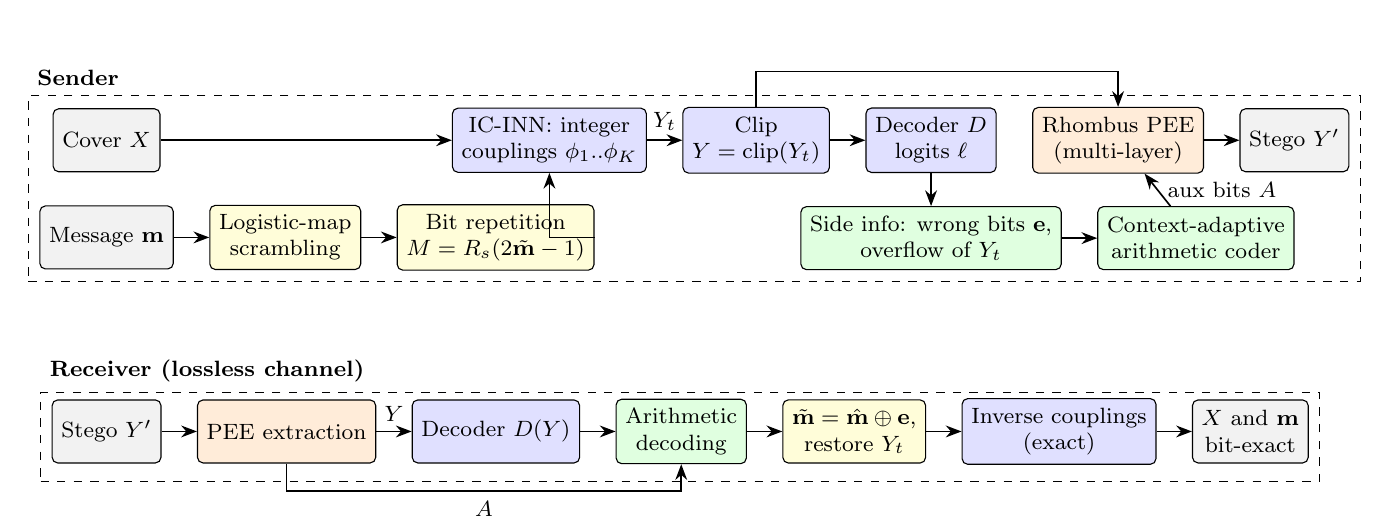
\begin{tikzpicture}[font=\footnotesize, node distance=0.42cm and 0.45cm,
  blk/.style={draw, rounded corners=2pt, align=center, minimum height=0.8cm, fill=#1},
  blk/.default=white, ar/.style={-{Stealth[length=2mm]}, semithick}]
% sender
\node[blk=gray!10] (cov) {Cover $X$};
\node[blk=gray!10, below=of cov] (msg) {Message $\mathbf{m}$};
\node[blk=yellow!15, right=of msg] (scr) {Logistic-map\\scrambling};
\node[blk=yellow!15, right=of scr] (map) {Bit repetition\\$M=R_s(2\tilde{\mathbf m}-1)$};
\node[blk=blue!12, right=1.1cm of cov, xshift=2.6cm] (cpl) {IC-INN: integer\\couplings $\phi_1..\phi_K$};
\node[blk=blue!12, right=of cpl] (clip) {Clip\\$Y=\mathrm{clip}(Y_t)$};
\node[blk=blue!12, right=of clip] (dec) {Decoder $D$\\logits $\ell$};
\node[blk=green!12, below=of dec] (side) {Side info: wrong bits $\mathbf e$,\\overflow of $Y_t$};
\node[blk=green!12, right=of side] (ac) {Context-adaptive\\arithmetic coder};
\node[blk=orange!15, right=of dec] (pee) {Rhombus PEE\\(multi-layer)};
\node[blk=gray!10, right=of pee] (st) {Stego $Y'$};
\draw[ar] (cov) -- (cpl);
\draw[ar] (msg) -- (scr); \draw[ar] (scr) -- (map); \draw[ar] (map) -| (cpl);
\draw[ar] (cpl) -- node[above]{$Y_t$} (clip); \draw[ar] (clip) -- (dec);
\draw[ar] (dec) -- (side); \draw[ar] (side) -- (ac); \draw[ar] (ac) -- node[right]{aux bits $A$} (pee);
\draw[ar] (clip.north) |- ++(0,0.45) -| (pee.north);
\draw[ar] (pee) -- (st);
\node[draw, dashed, inner sep=4pt, fit=(cov)(msg)(scr)(map)(cpl)(clip)(dec)(side)(ac)(pee)(st), label={[anchor=south west]north west:\textbf{Sender}}] {};
% receiver
\node[blk=gray!10, below=1.65cm of msg] (st2) {Stego $Y'$};
\node[blk=orange!15, right=of st2] (pee2) {PEE extraction};
\node[blk=blue!12, right=of pee2] (dec2) {Decoder $D(Y)$};
\node[blk=green!12, right=of dec2] (ac2) {Arithmetic\\decoding};
\node[blk=yellow!15, right=of ac2] (fix) {$\tilde{\mathbf m}=\hat{\mathbf m}\oplus\mathbf e$,\\restore $Y_t$};
\node[blk=blue!12, right=of fix] (inv) {Inverse couplings\\(exact)};
\node[blk=gray!10, right=of inv] (out) {$X$ and $\mathbf m$\\bit-exact};
\draw[ar] (st2) -- (pee2); \draw[ar] (pee2) -- node[above]{$Y$} (dec2); \draw[ar] (dec2) -- (ac2);
\draw[ar] (pee2.south) |- ++(0,-0.35) -| node[pos=0.25, below]{$A$} (ac2.south);
\draw[ar] (ac2) -- (fix); \draw[ar] (fix) -- (inv); \draw[ar] (inv) -- (out);
\node[draw, dashed, inner sep=4pt, fit=(st2)(pee2)(dec2)(ac2)(fix)(inv)(out), yshift=-2pt, label={[anchor=south west]north west:\textbf{Receiver (lossless channel)}}] {};
\end{tikzpicture}
\caption{System architecture of INN-RC. On a lossy channel the receiver only applies $D$ to the received image and reads
the message; the cover cannot be restored in that case.}
\label{fig:arch}
\end{figure*}

\subsection{Message-conditioned integer coupling}
The message is first XOR-ed with a keystream $\mathbf{k}$ from the logistic map $z_{t+1}=3.99\,z_t(1-z_t)$ seeded by a
secret key, $\tilde{\mathbf m}=\mathbf m\oplus\mathbf k$. Each bit is spread over an $s\times s$ block of the half-resolution
grid, giving the map $M=R_s(2\tilde{\mathbf m}-1)\in\{-1,1\}^{\frac H2\times\frac W2}$ and a payload of
$N=HW/(4s^2)$ bits, i.e. $1/(4s^2)$ bpp.

The cover is split by a $2\times 2$ space-to-depth into two halves, $X_a=[X(2i,2j),X(2i{+}1,2j{+}1)]$ and
$X_b=[X(2i,2j{+}1),X(2i{+}1,2j)]$. $K=4$ coupling steps then update one half from the other half and the message:
\begin{equation}
\begin{aligned}
X_b^{(k)} &= X_b^{(k-1)} + \big\lfloor \phi_k\big(X_a^{(k-1)}/255,\,M\big) \big\rceil, && k \text{ odd},\\
X_a^{(k)} &= X_a^{(k-1)} + \big\lfloor \phi_k\big(X_b^{(k-1)}/255,\,M\big) \big\rceil, && k \text{ even},
\end{aligned}
\label{eq:couple}
\end{equation}
where $\lfloor\cdot\rceil$ is rounding and $\phi_k(\cdot)=16\tanh(\tfrac12 f_k(\cdot))$, with $f_k$ three $3{\times}3$
convolutions (32 channels, leaky ReLU). The bound of $\pm16$ grey levels keeps training stable. Reassembling the halves
gives the integer stego $Y_t$, which may leave $[0,255]$ by a few levels, and the transmitted image is
$Y=\mathrm{clip}(Y_t,0,255)$.

Every step in (\ref{eq:couple}) is an integer addition whose increment depends only on the \emph{other} half and on $M$.
Hence, for a known $M$, the receiver inverts it exactly:
\begin{equation}
X_a^{(k-1)} = X_a^{(k)} - \big\lfloor \phi_k(X_b^{(k)}/255, M) \big\rceil \quad (k \text{ even}),
\label{eq:inv}
\end{equation}
and symmetrically for odd $k$, going from $k=K$ down to 1. No latent variable is produced, because the message is a
condition and not an input that has to come out on the other side.

\subsection{Message decoder and training}
A four-layer CNN $D$ takes the space-to-depth stego and outputs one logit per position of the half grid. Averaging over
each $s\times s$ block gives $\boldsymbol\ell\in\R^N$ and $\hat{\mathbf m}=\mathbb 1[\boldsymbol\ell>0]$. Coupling
networks and decoder (62{,}857 parameters in total) are trained jointly with
\begin{equation}
\begin{aligned}
\mathcal L ={}& \lambda_{\mathrm{img}}\,\overline{(Y-X)^2}
 + \lambda_{\mathrm{msg}}\,\mathrm{BCE}\big(\boldsymbol\ell(\mathcal N(Y)),\tilde{\mathbf m}\big)\\
 &+ \lambda_{\mathrm{of}}\,\overline{[-Y_t]_+ + [Y_t-255]_+},
\end{aligned}
\label{eq:loss}
\end{equation}
where $\mathcal N$ is a noise layer (identity with probability 0.45, otherwise Gaussian noise with
$\sigma\le 2$, salt-and-pepper up to 2\% or a $3\times3$ binomial blur) and the last term penalises overflow. Rounding
in (\ref{eq:couple}) is replaced by additive uniform noise~\cite{balle2017} in the first half of training and by the
straight-through estimator afterwards. The decoder first learns with $\lambda_{\mathrm{img}}\approx0$; the image and
overflow weights are then raised gradually. We train a quality-oriented model ($\lambda_{\mathrm{msg}}=10$) and a
robustness-oriented one ($\lambda_{\mathrm{msg}}=30$), each with $\lambda_{\mathrm{img}}=1$, $\lambda_{\mathrm{of}}=5$, and
one network serves $s\in\{2,4,8\}$.

\subsection{Residual compensation}
Two things separate the receiver from exact recovery: the bits where $\hat{\mathbf m}\neq\tilde{\mathbf m}$, and the
clipped pixels. The sender computes the error flags $\mathbf e=\hat{\mathbf m}\oplus\tilde{\mathbf m}$ from $D(Y)$, which the
receiver can reproduce, and for every pixel with $Y(p)\in\{0,255\}$ an overflow flag
$o_p=\mathbb 1[Y_t(p)\neq Y(p)]$, plus the magnitude $|Y_t(p)-Y(p)|$ when $o_p=1$. Flags are coded with an adaptive binary
arithmetic coder~\cite{witten1987ac}. The context of $e_i$ is the bin of $|\ell_i|$ among eight intervals
$[0,0.5,1,1.5,2,3,4,6,\infty)$, so its code length approaches
\begin{equation}
L_{\mathbf e}\approx\sum_i -\log_2 \hat P\big(e_i \mid c(|\ell_i|)\big),
\end{equation}
which is small because errors gather at low confidence. The context of $o_p$ is the pair (value 0 or 255, number of
4-neighbours at the same value). Magnitudes are Elias-gamma coded. The auxiliary stream $A$ is the 24-bit code length,
the arithmetic code and the magnitudes.

\subsection{Reversible embedding of the side information}
$A$ is hidden in $Y$ with rhombus PEE~\cite{sachnev2009}. Each pixel of one checkerboard set is predicted from its four
neighbours, $\hat y=\lfloor(y_u+y_d+y_l+y_r)/4\rceil$, and the error $\varepsilon=y-\hat y$ is changed to
\begin{equation}
\varepsilon'=\begin{cases}\varepsilon+1,&\varepsilon\ge1\\ \varepsilon+b,&\varepsilon=0\\ \varepsilon-b,&\varepsilon=-1\\
\varepsilon-1,&\varepsilon\le-2\end{cases}
\end{equation}
for a bit $b$. Pixels are visited in increasing order of local complexity and the second set is processed after the
first. If $A$ does not fit, further layers are added. Pixels whose prediction lies in $[1,4]$ or $[251,255]$ are skipped
(both sides can compute this), which prevents noisy black or saturated regions from overflowing; the few remaining
risky pixels are moved one level inwards and their positions are stored Elias-gamma coded in the pass header.

\begin{algorithm}[t]
\caption{Embedding}\label{alg:emb}
\begin{algorithmic}[1]
\Require cover $X$, message $\mathbf m$, key $\kappa$, repetition $s$
\State $\tilde{\mathbf m}\gets\mathbf m\oplus\mathrm{Logistic}(\kappa)$; $M\gets R_s(2\tilde{\mathbf m}-1)$
\State $(X_a,X_b)\gets\mathrm{S2D}(X)$
\For{$k=1$ to $K$} apply (\ref{eq:couple}) \EndFor
\State $Y_t\gets\mathrm{D2S}(X_a,X_b)$; $Y\gets\mathrm{clip}(Y_t,0,255)$
\State $\boldsymbol\ell\gets\mathrm{BlockMean}_s(D(Y))$; $\mathbf e\gets\mathbb 1[\boldsymbol\ell>0]\oplus\tilde{\mathbf m}$
\State $\Omega\gets\{p:Y(p)\in\{0,255\}\}$; $o_p\gets\mathbb 1[Y_t(p)\neq Y(p)],\ p\in\Omega$
\State $A\gets[\,|C|,\ C=\mathrm{AC}(\mathbf e,\mathbf o\mid\text{contexts}),\ \gamma(|Y_t-Y|_{o=1})\,]$
\State $Y'\gets\mathrm{PEE}(Y,A)$ \Comment{multi-layer rhombus PEE}
\State \Return stego $Y'$
\end{algorithmic}
\end{algorithm}

\begin{algorithm}[t]
\caption{Extraction and recovery}\label{alg:ext}
\begin{algorithmic}[1]
\Require stego $Y'$, key $\kappa$, repetition $s$
\State $(A,Y)\gets\mathrm{PEE}^{-1}(Y')$ \Comment{exact}
\State $\boldsymbol\ell\gets\mathrm{BlockMean}_s(D(Y))$; rebuild the contexts
\State decode $\mathbf e$, $\mathbf o$ and magnitudes from $A$; restore $Y_t$ from $Y$
\State $\tilde{\mathbf m}\gets\mathbb 1[\boldsymbol\ell>0]\oplus\mathbf e$; $M\gets R_s(2\tilde{\mathbf m}-1)$
\State $(X_a,X_b)\gets\mathrm{S2D}(Y_t)$
\For{$k=K$ down to $1$} apply (\ref{eq:inv}) \EndFor
\State \Return $X=\mathrm{D2S}(X_a,X_b)$, $\mathbf m=\tilde{\mathbf m}\oplus\mathrm{Logistic}(\kappa)$
\end{algorithmic}
\end{algorithm}

\newcommand{\ablA}{2747}
\newcommand{\ablB}{1869}
\newcommand{\ablC}{1589}
\newcommand{\ablD}{497}
\newcommand{\ablDicomC}{15325}
\newcommand{\ablDicomD}{2150}
\newcommand{\ablRatio}{5.5}
\newcommand{\ablRatioNb}{3.2}
\newcommand{\auxBASE}{111.7k}
\newcommand{\auxQeight}{365}
\newcommand{\auxQfour}{561}
\newcommand{\auxQtwo}{1659}
\newcommand{\auxRatio}{199}
\newcommand{\auxReight}{429}
\newcommand{\auxRfour}{610}
\newcommand{\auxRtwo}{928}
\newcommand{\berinnQeight}{0.44}
\newcommand{\berinnQfour}{3.04}
\newcommand{\berinnQtwo}{7.34}
\newcommand{\berinnReight}{0.23}
\newcommand{\berinnRfour}{2.05}
\newcommand{\berinnRtwo}{4.19}
\newcommand{\capPEE}{9.6k}
\newcommand{\exactBASE}{0}
\newcommand{\exactPEE}{393}
\newcommand{\exactQ}{385}
\newcommand{\exactR}{371}
\newcommand{\failBASE}{132}
\newcommand{\failPEE}{3}
\newcommand{\failQ}{11}
\newcommand{\failR}{25}
\newcommand{\nImgs}{132}
\newcommand{\okBASE}{0}
\newcommand{\okPEE}{393}
\newcommand{\okQ}{385}
\newcommand{\okR}{371}
\newcommand{\pinnBASE}{46.07}
\newcommand{\pinnQeight}{50.16}
\newcommand{\pinnQfour}{49.40}
\newcommand{\pinnQtwo}{46.64}
\newcommand{\pinnReight}{49.26}
\newcommand{\pinnRfour}{47.92}
\newcommand{\pinnRtwo}{43.49}
\newcommand{\psnrPEEeight}{71.64}
\newcommand{\psnrPEEfour}{65.32}
\newcommand{\psnrPEEtwo}{57.84}
\newcommand{\psnrQeight}{49.92}
\newcommand{\psnrQfour}{49.05}
\newcommand{\psnrQtwo}{45.73}
\newcommand{\psnrReight}{49.03}
\newcommand{\psnrRfour}{47.57}
\newcommand{\psnrRtwo}{42.94}
\newcommand{\resBASE}{36}
\newcommand{\robgaussonePEE}{50.17}
\newcommand{\robgaussoneQ}{2.07}
\newcommand{\robgaussoneR}{1.26}
\newcommand{\robgaussthreePEE}{50.05}
\newcommand{\robgaussthreeQ}{6.30}
\newcommand{\robgaussthreeR}{3.62}
\newcommand{\robgausstwoPEE}{49.87}
\newcommand{\robgausstwoQ}{3.22}
\newcommand{\robgausstwoR}{1.76}
\newcommand{\robjpegeightyPEE}{50.04}
\newcommand{\robjpegeightyQ}{47.02}
\newcommand{\robjpegeightyR}{46.10}
\newcommand{\robjpegnfPEE}{50.15}
\newcommand{\robjpegnfQ}{12.14}
\newcommand{\robjpegnfR}{5.07}
\newcommand{\robjpegninetyPEE}{50.47}
\newcommand{\robjpegninetyQ}{38.74}
\newcommand{\robjpegninetyR}{36.07}
\newcommand{\robnonezeroPEE}{0.00}
\newcommand{\robnonezeroQ}{1.78}
\newcommand{\robnonezeroR}{1.16}
\newcommand{\robspsphalfPEE}{48.29}
\newcommand{\robspsphalfQ}{3.35}
\newcommand{\robspsphalfR}{2.17}
\newcommand{\robspsponePEE}{48.99}
\newcommand{\robspsponeQ}{6.10}
\newcommand{\robspsponeR}{4.03}
\newcommand{\runsBASE}{132}
\newcommand{\runsPEE}{396}
\newcommand{\runsQ}{396}
\newcommand{\runsR}{396}
\newcommand{\ssimPEEeight}{0.9999}
\newcommand{\ssimPEEfour}{0.9998}
\newcommand{\ssimPEEtwo}{0.9991}
\newcommand{\ssimQeight}{0.9960}
\newcommand{\ssimQfour}{0.9949}
\newcommand{\ssimQtwo}{0.9896}
\newcommand{\ssimReight}{0.9955}
\newcommand{\ssimRfour}{0.9940}
\newcommand{\ssimRtwo}{0.9821}
\newcommand{\tembPEEeight}{0.02}
\newcommand{\tembPEEfour}{0.02}
\newcommand{\tembPEEtwo}{0.02}
\newcommand{\tembQeight}{0.49}
\newcommand{\tembQfour}{0.51}
\newcommand{\tembQtwo}{0.59}
\newcommand{\tembReight}{0.49}
\newcommand{\tembRfour}{0.51}
\newcommand{\tembRtwo}{0.56}
\newcommand{\textPEEeight}{0.02}
\newcommand{\textPEEfour}{0.02}
\newcommand{\textPEEtwo}{0.02}
\newcommand{\textQeight}{0.48}
\newcommand{\textQfour}{0.51}
\newcommand{\textQtwo}{0.59}
\newcommand{\textReight}{0.49}
\newcommand{\textRfour}{0.51}
\newcommand{\textRtwo}{0.56}

\section{Experimental Results and Analysis}
\subsection{Setup}
\textbf{Data.} Training uses the 100 Urban100 images~\cite{huang2015urban} converted to grey (92 for training, 8 for
validation) with random $64\times64$ crops and flips. Testing uses three sets that never appear in training: BSD100
\cite{martin2001bsd} ($256\times256$ centre crops), the 24 Kodak images~\cite{kodak} (grey, $512\times512$ centre crop
resized to $256\times256$, as is common practice for BOSSbase~\cite{bas2011boss}) and 8 real DICOM slices (3 CT, 2 MR,
2 CR, 1 perfusion CT) from the public pydicom test collection~\cite{pydicomdata}, windowed to 8 bits and resized to
$256\times256$. This gives \nImgs{} test images. BOSSbase 1.01 was not reachable from our network; the scripts accept
any folder of images.

\textbf{Training.} Both IC-INN models are trained for 12{,}000 iterations, batch 12, Adam~\cite{kingma2015adam} with a
cosine schedule from $10^{-3}$, on a 2-core CPU (about 15 minutes each). Fig.~\ref{fig:train} shows the curriculum: the
stego PSNR first drops while the decoder learns, then rises as the image loss is switched on.

\textbf{Compared methods.} (i) Rhombus PEE~\cite{sachnev2009} embedding the message directly, using our implementation
(the same one used for the side information). (ii) A float-INN baseline with residual compensation: a HiNet-style
\cite{jing2021hinet} affine-coupling network in the Haar domain (128.7k parameters), trained with rounding in the loop and
a cover-recovery loss; its residual $X-\lfloor 255\hat X\rceil$ and wrong bits are coded and hidden by PEE in the same way
as ours. (iii) IC-INN-Q and (iv) IC-INN-R, our quality- and robustness-oriented models.

\textbf{Metrics and payloads.} Payloads are 256, 1024 and 4096 bits ($s=8,4,2$), i.e.\ 0.0039, 0.0156 and 0.0625 bpp
of message on a $256\times256$ cover. We report PSNR and SSIM~\cite{wang2004ssim} of the final stego against the cover,
the side-information size, BER and NC of the extracted message, and whether the cover came back bit for bit. A run counts
as exact only if both \texttt{isequal(cover, recovered)} and \texttt{isequal(message, extracted)} hold in MATLAB.

\subsection{Reversibility and image quality}
Table~\ref{tab:main} lists the lossless results. Every run that finished embedding was exactly reversible:
\exactQ{} of \runsQ{} runs for IC-INN-Q and \exactR{} of \runsR{} for IC-INN-R, with BER $=0$ and NC $=1$ in all of them,
on natural and medical images alike. The remaining runs (\failQ{} and \failR{}) failed \emph{before} embedding because
the side information did not fit into the PEE capacity of the image; this happens only for busy textures or noisy dark
scans at the largest payload, and the sender detects it. Classical PEE fails on \failPEE{} runs for the same reason.

At 1024 bits IC-INN-Q reaches \psnrQfour{}~dB and SSIM \ssimQfour{}; at 4096 bits \psnrQtwo{}~dB and \ssimQtwo{}.
Before the side information is added the stego has \pinnQfour{} and \pinnQtwo{}~dB, so the compensation stage costs
less than 1~dB. The side information is smaller than the message it protects: on average \auxQfour{} bits for a
1024-bit message and \auxQtwo{} bits for a 4096-bit one. Fig.~\ref{fig:psnr} shows PSNR and side-information size against
payload, and Fig.~\ref{fig:visual} shows examples; the difference images are noise-like, with no visible structure.

Classical PEE gives much higher PSNR at these small payloads (\psnrPEEfour{}~dB at 1024 bits). This is expected and we do
not hide it: when the channel is guaranteed lossless, prediction-error expansion changes only a few hundred pixels by
one level, while a learned embedding spreads a decodable signal over the whole image. The point of the learned embedding
is what happens when the channel is \emph{not} lossless (Section~\ref{sec:robust}).

\begin{table*}[t]
\centering
\caption{Lossless results per test set and payload (mean over images). Aux = side-information bits embedded by PEE; Exact = images whose cover \emph{and} message were recovered bit for bit. Lossless BER was 0 and NC was 1 for every exact case.}
\label{tab:main}
\setlength{\tabcolsep}{3.2pt}
\begin{tabular}{lcc|ccc|cccc|cccc}
\toprule
& & & \multicolumn{3}{c|}{Rhombus PEE \cite{sachnev2009}} & \multicolumn{4}{c|}{IC-INN-Q (ours)} & \multicolumn{4}{c}{IC-INN-R (ours)}\\
Set & Bits & bpp & PSNR & SSIM & Exact & PSNR & SSIM & Aux & Exact & PSNR & SSIM & Aux & Exact\\
\midrule
BSD100 & 256 & 0.0039 & 71.30 & 0.9999 & 100/100 & 49.87 & 0.9971 & 310 & 99/100 & 48.96 & 0.9965 & 327 & 99/100\\
 & 1024 & 0.0156 & 64.91 & 0.9998 & 100/100 & 49.00 & 0.9960 & 459 & 99/100 & 47.52 & 0.9948 & 499 & 98/100\\
 & 4096 & 0.0625 & 57.24 & 0.9991 & 98/100 & 45.69 & 0.9904 & 1608 & 95/100 & 42.87 & 0.9827 & 980 & 89/100\\
\midrule
Kodak & 256 & 0.0039 & 71.98 & 0.9999 & 24/24 & 50.25 & 0.9966 & 334 & 24/24 & 49.33 & 0.9959 & 353 & 24/24\\
 & 1024 & 0.0156 & 65.88 & 0.9998 & 24/24 & 49.31 & 0.9954 & 438 & 24/24 & 47.79 & 0.9936 & 535 & 24/24\\
 & 4096 & 0.0625 & 58.70 & 0.9991 & 23/24 & 46.03 & 0.9895 & 1191 & 23/24 & 43.15 & 0.9797 & 731 & 22/24\\
\midrule
DICOM & 256 & 0.0039 & 74.77 & 1.0000 & 8/8 & 49.51 & 0.9799 & 1137 & 8/8 & 49.09 & 0.9820 & 1918 & 8/8\\
 & 1024 & 0.0156 & 68.78 & 0.9998 & 8/8 & 48.87 & 0.9802 & 2191 & 8/8 & 47.50 & 0.9817 & 2730 & 6/8\\
 & 4096 & 0.0625 & 62.63 & 0.9989 & 8/8 & 45.23 & 0.9738 & 4791 & 5/8 & 43.94 & 0.9789 & 640 & 1/8\\
\bottomrule
\end{tabular}
\end{table*}


\begin{figure}[t]
\centering
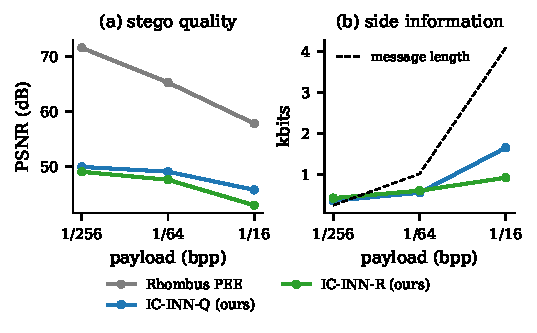
\includegraphics[width=\columnwidth]{figs/psnr_bpp.pdf}
\caption{(a) Mean stego PSNR over all test images versus payload. (b) Mean side-information size; the dashed line is
the message length.}
\label{fig:psnr}
\end{figure}

\begin{figure}[t]
\centering
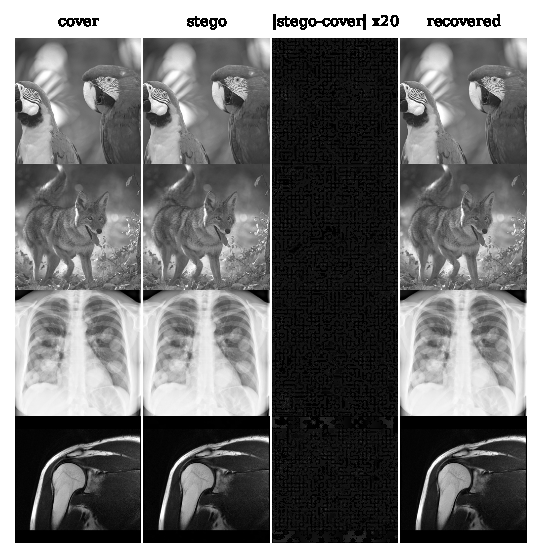
\includegraphics[width=0.92\columnwidth]{figs/visual.pdf}
\caption{IC-INN-Q at 1024 bits (Kodak 23, BSD100 \#10, chest CR, shoulder MR). The recovered images are identical to
the covers.}
\label{fig:visual}
\end{figure}

\subsection{Side-information coding (ablation)}
Table~\ref{tab:ablation} isolates the coder. Without entropy coding (A0) the side information averages \ablA{} bits at
1024-bit payload; a context-free arithmetic coder (A1) roughly halves it, and decoder-confidence contexts for the
message errors with neighbourhood contexts for the overflow flags (A2, our first version) give \ablC{} bits. The
predicted-offset contexts and coded magnitudes (A3) bring this down to \ablD{} bits, \ablRatioNb{}$\times$ smaller than
A2 and \ablRatio{}$\times$ smaller than A0. The gain comes almost entirely from the DICOM images, whose black
backgrounds produce thousands of overflowed pixels: there A2 needs \ablDicomC{} bits and A3 only \ablDicomD{}.

\begin{table}[t]
\centering
\caption{Mean side-information size (bits) for four coding choices. A0: raw flags; A1: arithmetic coding without contexts; A2: confidence contexts for message errors, neighbourhood contexts for overflow; A3: proposed (predicted-offset contexts, coded magnitudes).}
\label{tab:ablation}
\setlength{\tabcolsep}{4pt}
\begin{tabular}{llrrrr}
\toprule
Bits & Set & A0 & A1 & A2 & A3\\
\midrule
1024 & BSD100 & 1663 & 824 & 703 & 397\\
1024 & Kodak & 1716 & 806 & 703 & 365\\
1024 & DICOM & 19396 & 18108 & 15325 & 2150\\
1024 & All & 2747 & 1869 & 1589 & 497\\
4096 & BSD100 & 4843 & 2313 & 1938 & 1686\\
4096 & Kodak & 4898 & 2087 & 1724 & 1469\\
4096 & DICOM & 26542 & 22650 & 18292 & 8520\\
4096 & All & 6168 & 3504 & 2891 & 2061\\
\bottomrule
\end{tabular}
\end{table}


\subsection{Comparison with the float-INN baseline}
Table~\ref{tab:compare} summarises all methods at 1024 bits. The float-INN baseline hides the message well (its decoder
makes no errors and its stego has \pinnBASE{}~dB before compensation), but when the receiver inverts it with the latent
set to zero and the stego rounded to 8 bits, \resBASE\% of the cover pixels come back wrong. Coding that residual needs
\auxBASE{} bits on average, about \auxRatio{} times more than IC-INN-Q and far more than the
\capPEE{} bits a single PEE layer offers on these images, so not one of the \nImgs{} images could be embedded
reversibly. This is exactly the failure that motivated the integer, message-conditioned design: in IC-INN the cover
residual is zero by construction and only overflow and decoder errors remain.

\begin{table*}[t]
\centering
\caption{Comparison at 1024 bits (0.0156 bpp) over all test images. Success = embedding possible; Exact = cover and message recovered bit for bit; lossy-channel BER for Gaussian noise ($\sigma{=}2$) and 1\% salt-and-pepper noise. Times are MATLAB/Octave on a 2-core CPU. $^\dagger$PSNR of the INN stego before PEE; its side information never fits.}
\label{tab:compare}
\setlength{\tabcolsep}{4pt}
\begin{tabular}{lccccccccc}
\toprule
Method & Params & PSNR (dB) & SSIM & Aux (bits) & Success & Exact & BER GN2 (\%) & BER S\&P1 (\%) & Embed / extract (s)\\
\midrule
Rhombus PEE & 0 & 65.32 & 0.9998 & -- & 132/132 & 132/132 & 49.87 & 48.99 & 0.02 / 0.02\\
Float INN + RC (baseline) & 128.7k & 46.07$^\dagger$ & -- & 111.7k & 0/132 & 0/132 & -- & -- & -- \\
IC-INN-Q (ours) & 62.9k & 49.05 & 0.9949 & 561 & 131/132 & 131/132 & 3.22 & 6.10 & 0.51 / 0.51\\
IC-INN-R (ours) & 62.9k & 47.57 & 0.9940 & 610 & 128/132 & 128/132 & 1.76 & 4.03 & 0.51 / 0.51\\
\bottomrule
\end{tabular}
\end{table*}


\subsection{Robustness on a lossy channel}\label{sec:robust}
Table~\ref{tab:robust} reports the BER when the final stego is distorted before extraction (all Kodak and DICOM images
and the first 18 BSD100 images). Classical PEE loses everything: its extraction depends on exact pixel values, so its BER
is about 50\% under every attack. Our decoder reads the message directly from the received image. Without any attack it
already gets \robnonezeroR\% of the bits wrong (IC-INN-R), which is why the side information is needed for exact recovery;
under Gaussian noise with $\sigma=2$ the BER is \robgausstwoR\% and under 1\% salt-and-pepper noise \robspsponeR\%. Mild
JPEG compression (quality 95) gives \robjpegnfR\%, but quality 90 or lower destroys the message (\robjpegninetyR\%), which is
not surprising since JPEG was not part of the noise layer. The robustness-oriented model is consistently better than the
quality model, at the cost of 1.5~dB.

\begin{table}[t]
\centering
\caption{Message BER (\%) on a lossy channel, payload 1024 bits, 50 images. The cover is not recoverable here; the question is only how many message bits survive.}
\label{tab:robust}
\setlength{\tabcolsep}{4pt}
\begin{tabular}{lcccc}
\toprule
Attack & PEE & Float INN & IC-INN-Q & IC-INN-R\\
\midrule
none & 0.00 & -- & 1.78 & 1.16\\
GN $\sigma{=}1$ & 50.17 & -- & 2.07 & 1.26\\
GN $\sigma{=}2$ & 49.87 & -- & 3.22 & 1.76\\
GN $\sigma{=}3$ & 50.05 & -- & 6.30 & 3.62\\
S\&P 0.5\% & 48.29 & -- & 3.35 & 2.17\\
S\&P 1\% & 48.99 & -- & 6.10 & 4.03\\
JPEG 95 & 50.15 & -- & 12.14 & 5.07\\
JPEG 90 & 50.47 & -- & 38.74 & 36.07\\
JPEG 80 & 50.04 & -- & 47.02 & 46.10\\
\bottomrule
\end{tabular}
\end{table}


\subsection{Complexity}
The coupling networks have 42{,}888 parameters and the decoder 19{,}969. Embedding and extraction take about
\tembQfour{}~s each for a $256\times256$ image in our MATLAB code (Octave, single CPU core), of which most is the inverse
pass and the arithmetic coder. Classical PEE takes about 0.02~s. The GUI (\texttt{INNRC\_App.m}) runs the same functions
interactively.


\section{Conclusion and Future Scope}
We presented INN-RC, a lossless steganography scheme in which an integer coupling network is conditioned on the
message instead of taking it as an input. Because every coupling step is an integer addition driven by the other pixel
half and the message, the cover is recovered exactly once the message is known, and the only residual that has to be
compensated is the set of wrongly decoded bits and the clipped pixels. Coding this residual with contexts the receiver
can rebuild (decoder confidence and the re-estimated coupling offset) keeps it smaller than the message itself.

\textbf{Exact reversibility.} In all \exactQ{} successful IC-INN-Q runs and \exactR{} IC-INN-R runs on \nImgs{} test
images, the recovered cover was identical to the original pixel for pixel and the extracted message had BER $=0$
(NC $=1$), which we verified with \texttt{isequal} in MATLAB rather than with a PSNR threshold.

\textbf{Limitations.} (i) On a guaranteed lossless channel classical PEE still gives a higher PSNR at these payloads;
our scheme pays for robustness with image quality. (ii) At 4096 bits a few busy or noisy dark images cannot hold the
side information and embedding is refused. (iii) The receiver must reproduce the rounded coupling offsets exactly, so
sender and receiver should run the same floating-point code; a fixed-point network would remove this assumption.
(iv) We work on 8-bit grayscale images and converted the DICOM scans to 8 bits, and BOSSbase could not be included.

\textbf{Future work.} Fixed-point (integer-only) coupling networks for platform-independent decoding, native 12/16-bit
DICOM and colour images, a learned predictor for the PEE stage to increase its capacity, larger payloads through a
multi-scale message map, and testing against deep steganalysers.


\bibliographystyle{IEEEtran}
\bibliography{refs}

\end{document}
